\documentclass[11pt, oneside]{article}   	% use "amsart" instead of "article" for AMSLaTeX format
\usepackage{geometry}                		% See geometry.pdf to learn the layout options. There are lots.
\geometry{letterpaper}                   		% ... or a4paper or a5paper or ... 
%\geometry{landscape}                		% Activate for rotated page geometry
%\usepackage[parfill]{parskip}    		% Activate to begin paragraphs with an empty line rather than an indent
\usepackage{graphicx}				% Use pdf, png, jpg, or eps§ with pdflatex; use eps in DVI mode
								% TeX will automatically convert eps -> pdf in pdflatex		
\usepackage{amssymb}
\usepackage{hhline}
\usepackage{amsmath}
%SetFonts
\usepackage{csquotes}
\usepackage{multirow}
\usepackage{booktabs}

\usepackage{multirow}
\usepackage{tabularx}
\usepackage{ragged2e}
\usepackage[colorlinks]{hyperref}
\hypersetup{colorlinks=true,linkcolor=blue,urlcolor  = blue,citecolor = blue}

%SetFonts


\title{Training LLMs on Simple, Safe Text}
%\date{}							% Activate to display a given date or no date

\begin{document}
\maketitle
\tableofcontents
\section{Introduction}

In this project we will explore how to build a LLM that answers questions in a simple and safe ($S^{2}$) way.
That is, we want an LLM which answers questions in a way which is understandable to schoolchildren and/or adults who are learning English while also not producing any potentially toxic or offensive content.
To train the LLM we will use a combination of imitation learning and preference modeling.
The two main algorithms we will explore are Reinforcement Learning from Human Feedback (RLHF) \cite{ouyang2022training,bai2022training} and Direct Preference Optimization (DPO) \cite{rafailov2023direct}. 

In the remainder of this introduction we will briefly review these methods.
We will attempt to be light on the mathematical details of the algorithms and instead focus on the overall challenges and benefits of each approach.
 
 \subsection{RLHF}
RLHF is the most well-known method used to align LLMs with human interests and is behind the success of chatbots such as ChatGPT and Claude.
RLHF is roughly given by the following three step procedure:
\begin{enumerate}
\item We start by training the model using supervised fine-tuning (SFT). At this step we simply prompt the model with a question in the form ``\#\#\# Human: \{question\} \#\#\#Assistant:" and ask the model to autoregressively generate new text. This is called supervised fine-tuning because we have a reference human-written answer and want to minimize the KL-divergence between the reference text and the model generated text. Despite its name, SFT is essentially the same as pretraining, except we do not compute the loss on the prompt.

\item Next, we perform reward modeling (RM), which is a preference modeling task.
In this step, we take another neural net and present it with a question and two answers, one of which is labelled ``chosen" and the other one is labelled ``rejected".
At this step, the goal is to teach the model to identify which answer is preferred over the other, i.e. to learn human preferences via sequence classification. 
Typically the reward model is taken to be the LLM from step (1), but we replace the head of the SFTed model with a layer to compute the reward function $r(Q,A)$ and train the model with a loss function such that the model assigns higher rewards to the chosen answer and lower rewards to the rejected answer. 

\item Finally, we use the reward model from step (2) to train the SFTed model from step (1) using reinforcement learning.
Specifically, the model is trained using Proximal Policy Optimization (PPO).
At this step it helps to add a term to the reward modeling objective proportional to the KL-divergence between the SFT model we are training and the original SFT from step (1).
The addition of a KL penalty helps ensure that the model trained with RL does not deviate too strongly from the original model and produce low-quality text that simply ``hacks" the reward model.
\end{enumerate}

To be more precise, during step (2) we typically assume that human preferences are captured by the Bradley-Terry model:
\begin{align}
p^{*}(y_1\succ y_1|x)=\frac{e^{r^{*}(x,y_1)}}{e^{r^{*}(x,y_1)}+e^{r^{*}(x,y_2)}}
\end{align}
where $r^{*}$ is the gold reward model.
To find the optimal reward model we can minimize the following loss function:
\begin{align}
\mathcal{L}(r_{\phi},\mathcal{D}) = - \mathbb{E}_{(x,y_{w},y_{l})\sim\mathcal{D}}\left[\log(\sigma(r_{\phi}(x,y_w)-r_{\phi}(x,y_l)))\right]
\label{eq:reward_optimization}
\end{align}
where $\phi$ are the parameters of the reward model, $y_w$ and $y_l$ are the chosen/rejected answers, respectively, $\mathcal{D}$ is our dataset, and $\sigma$ is the logistic function. 

During the RL step the goal is to find a policy (LLM) $\pi_{\theta}$ which solves the following optimization problems:
\begin{align}
\pi_{\theta^{*}} = \text{argmax}_{\pi_{\theta}}\mathbb{E}_{x\sim \mathcal{D},y\sim \pi_{\theta}(y|x)}[r_{\phi}(x,y)]-\beta \mathcal{D}_{KL}[\pi_{\theta}(y|x)||\pi_{\text{\text{ref}}}(y|x)]
\label{eq:constrained_optimization}
\end{align}
where $r_{\phi}$ is the previous learned reward model, $\mathcal{D}_{KL}$ is the KL-divergence, and $\pi_{\text{\text{ref}}}$ is the SFT model from step (1).
The parameter $\beta$ is a hyperparameter which controls how much we penalize deviations from the original reference model.
The optimal policy is then found using PPO.

RLHF is clearly a non-trivial algorithm to implement in practice. 
The simplest step to implement is the SFT since the training objective is essentially identical to the pretraining objective. 
In addition, if we have a dataset of high enough quality, we arguably do not need to perform many steps of supervised fine-tuning, e.g. in the LIMA paper they achieved remarkable after only training the model with SFT on 1000 examples!

The second step, reward modeling, is simple to implement in principle, but in practice can be very subtle and difficult to get right.
For one, we are trying to teach a model what human preferences are by simply ranking two answers.
This may be too rough of a metric to actually determine human preferences, e.g. what answer is preferred over the another may depend on how the question is written and who the intended audience is.
In addition, what answer is considered the ``best" will be biased by the preferences of whoever is ranking the answer, and their preferences may not be universal.
%On internet sites, such as Reddit, one answer may also receive more votes than another simply because it appeared earlier, and not because it is of a genuinely higher quality.
In theory, it may also be better to have multiple reward models to judge different aspects of an answer, as opposed to having one reward model which is supposed to determine the quality of the answer in full.\footnote{We may want separate reward models to separately judge the simplicity, helpfulness, and harmfulness of the answer.}
However, despite its simplicity, learning human preferences by ranking answers has proven remarkably successful and is also a natural starting point for solving the alignment problem.
%All that being said, one reason why training a reward model on data from sites such as Reddit or StackExchange is useful is because actually getting human preference data is non-trivial and these sites give us access to both a wide scope of data on which we can get started.
%In addition, by using the ``Wisdom of the crowd" of users who vote on answers, we can potentially avoid biasing the data by the preferences of a small group of labellers (of course the demographics of users on these sites is also biased towards certain groups and this should also be taken into account).

To successfully perform reward modeling, we also need to ensure that our preference dataset is of a high-enough quality such that we can use our trained reward model during the reinforcement learning step.
The general wisdom currently is that the reward model needs to be achieving accuracies of around $70\%$ (and ideally higher) before we can use it for reinforcement learning.
The fact these accuracies are fairly low is a testament to the fact that reward modeling by itself is a non-trivial task!
We also need to ensure the preference modeling dataset is of a wide enough scope such that the reward model knows how to properly judge answers that are generated during reinforcement learning.
For example, a model trained only to judge answers about math may not accurately judge answers about other topics, such as history or politics.

The final step of RLHF, implementing PPO, is more technically challenging than the previous steps.
The PPO algorithm requires that we have a value function, a reward model, the policy function (the LLM currently being trained), and the initial SFTed model (which serves as our reference model). 
Therefore, during PPO we have to keep four separate models in models, and they are all LLMs!
For this reason, the PPO step can be fairly memory intensive.
To avoid out-of-memory errors, and also spending too much money on GPUs, we either need to use relatively small LLMs and/or use parameter efficient methods such as QLoRA.
In addition, it is well-known that training a model with RL is more difficult than training a model using supervised learning and that RL algorithms tend to be more sensitive to hyperparameters and choices of initialization.
For this reason, we RL typically requires more hyperparameter optimization than supervised or unsupervised learning.

\subsection{DPO}
DPO is a newer algorithm designed to achieve the same objective as RLHF using only supervised learning.
DPO is a supervised learning algorithm that optimizes the same objective as RLHF, except without needing to train a separate reward model (hence the subtitle of the paper, ``Your Language Model is Secretly a Reward Model") and without needing to perform reinforcement learning.
To do this, they use an exact map between reward functions to optimal policies such that the loss function on the reward model becomes a loss function on the policy model.
Therefore, step (2) of the RLHF algorithm, performing supervised learning on the reward model, turns into a supervised learning problem on the policy function directly, which in our case is the SFTed LLM.

DPO is therefore a two step procedure:
\begin{enumerate}
\item Perform supervised fine-tuning on a pre-trained LLM in the same exact way as step one of RLHF.
\item Take the model from step (1) and train it to learn human preferences directly using the DPO loss function.  
\end{enumerate} 

To proof that the DPO is equivalent to RLHF, they first show that the optimal policy which satisfies equation \ref{eq:constrained_optimization} is:
\begin{align}
\pi_{r}(y|x)=\frac{1}{Z(x)}\pi_{\text{ref}}(y|x)e^{\frac{r(x,y)}{\beta}}
\end{align} 
where the partition function is:
\begin{align}
Z(x)=\sum\limits_{y}\pi_{\text{ref}}(y|x)e^{\frac{r(x,y)}{\beta}}.
\end{align}
After making this identification, the reward modeling step, equation \ref{eq:reward_optimization}, becomes equivalent to minimizing the following loss function:
\begin{align}
\mathcal{L}_{\text{DPO}}(\pi_{\theta};\pi_{\text{ref}}) = -\mathbb{E}_{(x,y_w,y_l)}\sim\mathcal{D}\left[\log \sigma \left(\beta \log \frac{\pi_{\theta}(y_w|x)}{\pi_{\text{ref}}(y_w|x)}-\beta \log \frac{\pi_{\theta}(y_l|x)}{\pi_{\text{ref}}(y_l|x)}\right)\right]
\end{align}

DPO is overall a simpler algorithm to implement and use since it just involves supervised learning.
For this reason, we will start by using DPO to align our LLMs and use the results from DPO as a benchmark for RLHF. 
In the original DPO paper it was also shown that DPO achieves comparable or better results than RLHF, so we expect DPO will serve as a strong benchmark for RLHF, or any other algorithm to align LLMs. 

Are there any downsides to DPO?
One potential downside, given its current incarnation, is that there may be cases where we want a separate reward model.
This is brought up in the DPO paper, where they mention that having a separate reward model may be useful to label currently unlabelled prompts, and it is less clear if performing self-labelling using the LLM (which is also being trained) is equally effective.
In addition, as brought up earlier, it may be useful to have multiple reward models to capture different aspects of an answer, e.g. helpfulness vs simplicity. 
This theoretically can be implemented in RLHF by simply training more reward models, but it is not clear how to do this using DPO directly since in DPO our LLM is also the reward model.
Finally, like most implementations of RLHF, the DPO algorithm assigns a single score to an entire answer and does judge individual parts of the answer.

\section{Datasets}

\subsection{Sources}
The two sources of our datasets are the ELI5 dataset and Simple Wikipedia.
In this section we will go into detail on the form of these datasets and in the next section we will explain how we filtered them. 

\subsubsection*{ELI5}

The ELI5 dataset gets its name from the subreddit Explain Like I'm Five (r/ELI5) on reddit.com.
The stated goal of the ELI5 subreddit is to provide a place where people can ask questions on a wide variety of topics and receive a layperson-friendly explanation.
Commentators are requested to answer a question without assuming ``knowledge beyond a typical secondary education program" and in general to keep answers clear and simple.
The ELI5 dataset also contains question/answer pairs from the r/AskHistorians and r/AskScience subreddits. The r/AskHistorians is well-known to be a well-moderated community where answers are particularly in-depth and clear. 
Low quality answers, e.g. ones that do not answer the original question or do not properly cite sources, are typically removed.
The quality of posts on r/AskScience is also high and users generally receive clear answers to fairly technical questions, although the moderation appears to be less strict than on r/AskHistorians.
We will use the ELI5 dataset to train a question/answer model by using the title and body of the post as the question and highly-voted comments as the answers.

The original ELI5 dataset was created by researchers at Facebook \cite{fan-etal-2019-ELI5} and the original ELI5 dataset can be found \href{https://huggingface.co/datasets/ELI5}{here}.
However, one potential issue with this dataset is that there is a large amount of data leakage between the train/validation/test splits \cite{krishna2021hurdles,mahapatra2021new}.
For this reason, we will use a cleaned version of the ELI5 dataset which was constructed by the second group and can be found \href{https://huggingface.co/datasets/vblagoje/lfqa}{here}.
This dataset will also require some cleaning due to data leakage, but overall its cleaner than the previous version of the ELI5 dataset.


\subsubsection*{Wikipedia}
\href{https://simple.Wikipedia.org/Wiki/Main_Page}{Simple Wikipedia} is a version of Wikipedia where users are encouraged to write articles using basic English.
On the Simple Wikipedia homepage they write: ``The Simple English Wikipedia is for everyone, such as children and adults who are learning English."
They also encourage users to write shorter sentences, while not necessarily requiring that the articles also be short.
In particular, users are told to write articles using simple words and grammar, but to not necessarily only use ``basic information".
Unlike the ELI5 dataset, we cannot use the Simple Wikipedia dataset out of the box to train a question-answering model since the articles are not written in that style.
Instead, we will use GPT-3.5 to generate questions whose answer is contained in the first few paragraphs of the Simple Wikipedia article \cite{koksal2023longform}. 
Specifically, we give GPT-3.5 the following system message and prompt:
\\[5pt]
\indent \textbf{System Message}: ``You are a helpful assistant that generates questions from text."
\indent \textbf{Prompt}: ``Question: X
\newline
\indent\indent\indent\indent Answer: \{answer\} 
\\
\indent\indent\indent\indent What kind of question, X, could this be an answer to?\newline \indent\indent\indent\indent X:"
\\[5pt]
Here the text in \{answer\} is the first few paragraphs of the Simple Wikipedia article.

This is a very general and powerful idea which allows us to use large LLMs to generate whole new, synthetic datasets from existing text.
A nice feature of this method is that only the question is AI-generated, the answer itself is still human-written text which has been repurposed for a new task.
A dataset of Simple Wikipedia articles is hosted on HuggingFace \href{https://huggingface.co/datasets/Wikipedia/viewer/20220301.simple/train}{here} which we will use to generate the questions.

\subsection{Creating and Filtering the Datasets}
RLHF involves three separate training steps, supervised fine-tuning, reward modeling, and reinforcement learning, so we therefore need three separate datasets.
Each dataset also has its own train, validation, and test sets.
To perform DPO we also need separate datasets for supervised fine-tuning and reward modeling.
In this section we will summarize how we filter and split our initial dataset into these three datasets.
\subsubsection{ELI5}
The initial training, validation, and test splits of the \href{https://huggingface.co/datasets/vblagoje/lfqa}{ELI5} dataset contains 226147, 3020, and 10000 separate posts. 
However, each post can contain multiple question/answer pairs.
If we count each QA pair as a separate datapoint then the train, validation, and test splits contain 669139, 22636, and 41650 datapoints, respectively.

Before we split this dataset up into SFT/RM/RL subsets, we first performed some data cleaning.
To form the SFT and RM datasets we used the following procedure:
\begin{enumerate}
\item First we used \href{https://pypi.org/project/redditcleaner/}{redditcleaner} to remove Reddit-specific markdown formatting.
\item Next we removed any quoted texts in the answers. Although quoting the original question is not problematic in and of itself, we did this to shorten the answer and ensure the entire answer can fit in the context length.
\item We also removed any extra whitespaces from the text.
\item The ELI5 dataset uses the string ``\_url\_i\_" as a placeholder for URLs, which are stored elsewhere in the dataset. 
We decided to remove URLs given the propensity of LLMs to hallucinate fake sources.
Instead, we intend to use retrieval augmented generation (RAG) so our LLMs can properly cite sources.
\item We removed any answers which are less than 20 words long, since these tend to be uninformative. 
\item We removed any posts that did not fit the question answer paradigm, e.g. if the title/post did not actually contain a question.
There are many posts on these subreddits of these forms, e.g. r/AskScience has \href{https://www.reddit.com/r/askscience/comments/10wyuf9/ask_anything_wednesday_engineering_mathematics/}{``Ask Anything Wednesday"} posts where users ask questions and receive answers in the comments and r/AskHistorians has had meta posts on the state of the subreddit, see e.g. this \href{https://www.reddit.com/r/AskHistorians/comments/yfs7uh/askhistorians_has_hit_15_million_subscribers_to/}{post} celebrating the subreddit hitting 1.5 million subscribers. We manually went through the ELI5 dataset to identify and remove such posts.
\item We removed answers which did not meet our simplicity criteria according to the \href{https://en.Wikipedia.org/Wiki/Flesch\%E2\%80\%93Kincaid_readability_tests}{Flesch-Kincaid readability metrics}. Specifically, we measured the simplicity of an answer by computing its Flesch reading ease (FRE) and Flesch-Kincaid grade level (FKG) scores. We only kept posts with FRE$\geq 60$, which corresponds to ``simple English" and FKG$< 9$, which corresponds to text which should be understandable by middle-school students and younger (the FKG score approximately corresponds to US school grade level). 
\end{enumerate}

There is of course freedom to change the above data cleaning procedure and it would be interesting to explore alternatives. 
In particular, it may be useful to keep the quoted text in the answer so that our LLM learns that it's useful to quote the original text when replying.
In addition, keeping the URLs in the answer may not cause anymore hallucination than normal. 
Both options are certainly worth exploring in the future.

Of all of the above filtering steps, the last one is likely the most unique to our project. 
The Flesch-Kincaid readability metrics are automatic metrics developed in the 1970s to measure the difficulty of the text.
They are computed as follows:
\begin{align}
\text{FRE} &= 206.835-1.015\left(\frac{\text{total words}}{\text{total sentences}}\right)-84.6\left(\frac{\text{total syllables}}{\text{total words}}\right)
\\
\text{FKG} &= 0.39\left(\frac{\text{total words}}{\text{total sentences}}\right)+11.8\left(\frac{\text{total syllables}}{\text{total words}}\right)-15.59
\end{align}
It would of course be interesting to consider more advanced methods to determine the simplicity or complexity of a text.
For example, we can try to train a model to classify texts into different categories or we could simply prompt GPT-4.
We decided to use Flesch-Readability metrics because they both serve as a strong baseline to compare against more complicated models and also because they gave us a fast and easy way to filter our large datasets. 
We expect that more advanced methods may be more useful to perform further pruning of our dataset.

After applying the above filtering steps, we split the resulting dataset into the SFT and RM dataset.
If we want to use a post for reward modeling we of course need to ensure that it contains more than one answer!
For this reason, we put any post that only has one answer into the SFT dataset.
In addition, even if we have multiple answers, we also need clear human preferences between those answers.
Therefore, we only keep answers in the RM dataset if they have unique scores such that we can rank them.
If two answers have the same score, we move one of the answers (with the corresponding question) to the SFT dataset.  
Finally, we place any question which has not been placed into either the SFT or RM dataset into the reinforcement learning dataset.
Note that this includes questions which were filtered out in the above pre-processing steps since for RL we only need the questions, and not the answers, since the model's generation will be judged solely by the reward model and will not be compared to the human-written text. 
For DPO we will only use the SFT and RM datasets.

Once we have split the dataset into the SFT, RM, and RL datasets, we next need to ensure that each dataset does not have any data leakage.
To catch data leakage, we used the ``all-mpnet-base-v2" \href{https://www.sbert.net/}{SentenceTransformers} model to embed each question into a 768-dimensional vector space.\footnote{Specifically, we combined the title and body of the post into one string applied the SentenceTransformer model to that text.}
We then computed the cosine-similarities between the embedding vectors in the train, validation, and test sets. As a reminder, the cosine similarity is defined by:
\begin{align}
\text{cos-similarity}(v_1,v_2)=\frac{v_1\cdot v_2}{|\!|v_1|\!|_2 |\!|v_2|\!|_2},
\end{align}
where $|\!|\ |\!|_2$ is the standard $L_2$ norm.
After inspecting various questions and their cosine-similarity, we decided to use 0.6 as our cutoff for detecting data-leakage, i.e. if \\ $\text{cos-similarity}(v_1,v_2)\geq 0.6$ we would remove either $v_1$ or $v_2$.
If a training example overlapped significantly with an example in the validation or test sets, we removed it from the training set since the training dataset is much larger than the other two datasets.
For the same reason, if an example in the test set overlapped significantly with a vector in the validation set, we removed it from the test set. After removing data leakage, the cleaning process for the SFT and RM datasets starts to differ slightly, so we will consider these two datasets separately for the remained of this section.
\\[10pt]
{\large \textbf{Supervised Fine-Tuning}}
\\[10pt]
During supervised fine-tuning we are essentially teaching our model to imitate how humans (or more advanced LLMs) answer questions.
To avoid our model imitating bad behavior, we need to perform extra filtering steps.
As a first, basic filtering step, we only kept answer which received a score of at least 4 from the Reddit community. 
The original ELI5 dataset was constructed by only keeping posts that had a score of at least 2 and also contained answers with a score of at least two.

Next, to prevent the model from outputting toxic or offensive content, we used \href{https://github.com/unitaryai/detoxify}{Detoxify} from UnitaryAI to detect toxic content.
Specifically, we use the ``unbiased" model which has a RoBERTa-Base model fine-tuned on the dataset from the following \href{https://www.kaggle.com/c/jigsaw-unintended-bias-in-toxicity-classification}{Kaggle competition}. This competition defined toxic content to be anything that is ``rude, disrespectful or otherwise likely to make someone leave a discussion." 
The model from Detoxify scores assigns a score of 0-1 on the following 6 metrics: severe\_toxicity, obscene, threat, insult, identity\_attack, sexual\_explicit".
Higher scores are associated to toxic text while lower scores are associated with safer text.
We filtered by SFT dataset to only keep answers which received a score of $\leq 0.1$ on all six metrics.


After performing the above cleaning steps, we trained Llama-2 models on the SFT dataset.
However, we noticed some issues with the model's generated text at inference time.
In particular, the model had a tendency to end its posts with strings of text of the form: ``Edit: typos, Edit 2: Sorry caught more typos etc.". 
Evidently, the model picked up on the fact that many Reddit posts by adding edits either correcting information in the post, adding additional sources, or thanking other users.
To avoid our model learning this behavior, we filtered the SFT dataset to remove any answers which ended in this way. 

The final ELI5-SFT dataset contains a total of 41568 questions where the train\/validation\/test split is 38595/880/2093. 
\\[10pt]
{\large \textbf{Reward Modeling}}
\\[10pt]
For reward modeling we do not need to perform the same filtering steps as in SFT since we are now teaching the model to distinguish between good and bad responses.
Therefore, we do not necessarily need to filter out all answers with a low score or which contain toxic content, we just need to ensure these answers are always in the ``rejected" column. 
Similarly, we can also keep answers which end in "edit: caught typos" as long as they are also restricted to the rejected answer.

When we originally performed DPO, we did not apply the above procedure: we kept answers with low scores, but we also filtered out all toxic content and did not filter out answers that end with superfluous edits. 
We therefore need to repeat the DPO data cleaning and training procedure and will update this section once that has been completed.

In addition, we also have freedom about which answers to keep in the reward modeling dataset.
Recall that during the reward modeling step we typically perform a binary classification task.
Therefore, if a question receives 10 different answers we can construct 45 different chosen/rejected pairs. In general, if we have $n$ answers then we have n(n-1)/2 number of pairs. One simple option is to treat pair independently. 
However, it was pointed out in \cite{ouyang2022training} that doing this leads to overfitting since the model sees some questions much more frequently than other ones.
To avoid this issue we will explore the following options:
\begin{enumerate}
\item For each question only keep one pair of answers. We can choose to keep the top two answers, the answers with the highest/lowest number of votes, or two random answers.
By only keeping one pair of answers, we avoid overfitting, but we also throw out potentially useful data.
\item For each question, we keep multiple pairs of answers, but rescale the loss function so that question/answer pairs are weighted inversely proportional to how many answers a question received.
\end{enumerate}
The second option was used in \cite{ouyang2022training} where the loss function is:
\begin{align}
\mathcal{L}_{\theta}=-\frac{1}{{K\choose 2}}\mathbb{E}_{(x,y_w,y_l)\sim \mathcal{D}}\left[\log \sigma\left(r_{\theta}(x,y_w)-r_{\theta}(x,y_l)\right)\right].
\end{align}
To be truly efficient, one should compute the reward associated to each answer separately, combine the result in a large vector, and then compute the pairwise differences between all the possible accepted/rejected columns.
Given our memory limits and the size of the ELI5 QA pairs we cannot fit all the question/answer pairs into memory, so we will compute the loss on each pair separately.
In addition, we will only keep a maximum of 10 pairs for each answer.

\subsubsection{Simple Wikipedia}

For Simple Wikipedia the data cleaning procedure is relatively simpler than for ELI5.
Unlike for ELI5, all the QA pairs will be placed in the SFT dataset.
The reason is simply that to perform reward modeling, we need to have two answers to compare against.
At the moment we only have a single answer, text from the original Simple Wikipedia article, associated to each GPT-3.5 generated question, so we cannot perform any preference modeling, although there are ways around this we are exploring.
In addition, the Simple Wikipedia is written in an encyclopedic format, so the articles do not contain toxic content.

All that said, we still need to clean the original Simple Wikipedia dataset before we actually use GPT-3.5 to generate questions or perform any fine-tuning.
The original Simple Wikipedia dataset contains a total of 205328 articles which have not been split up into train/validation/test datasets.
We then apply the following filtering steps:
\begin{enumerate}
\item We remove any articles which are less than 50 words long. Articles shorter than 50 words tend to be fairly uninformative.
\item We define a ``truncated\_text" column which is defined to be the first few paragraphs of an article.
To create the truncated article we concatenate paragraphs from the original article until the truncated article is at least 300 words long. After it reaches 300 words, or we reach the end of the original article, we stop adding new text. The truncated text will be our ``answer" when training the question-answering model.
\item To avoid excessively long answers, we remove any answers which are more than 500 words long. This is done to ensure that the answers are both long-form and coherent.
\item We compute the Flesch Readability Ease (FRE) and Flesch-Kincaid grade score (FKG) and only keep articles which have an FRE$\geq 60$ and a FKG$<9$.
This is the same simplicity criteria as used for the Reddit data.
\item Finally, we split the resulting dataset into train/validation/test sets where the validation and test sets contain 5000 articles and the training set contains the remaining articles.
\end{enumerate}

After applying the above filtering steps, we noticed some articles contained text which was not written in natural language. 
Specifically, Wikipedia contains its own special markdown text for images and tables. 
We therefore removed any articles which contained such text to avoid confusing the LLM.
The resulting train/validation/test split of the Simple Wikipedia dataset contains 65254/4991/4997 articles.
We then used GPT-3.5 to create questions whose answers are given in the truncated articles to create the Simple Wikipedia SFT dataset.

\subsection{Exploratory Data Analysis}
This section will be filled in with more details on the features of our datasets.

\section{Inference}

\subsection{How to Define The Inference Model}
As is well-known, after training a model we have to make sure it is in ``evaluation" mode before performing inference, i.e. in PyTorch we call model.eval() to turn off dropout, prevent the accumulation of any more gradients, etc.

In this project we faced an additional subtlety because we used QLoRA to fine-tune the large language models.
In the original LoRA paper \cite{hu2021lora} they showed that one can efficiently fine-tune LLMs by adding low-rank adapter layers to the transformer.
Specifically, they added adapter weights to the query, key, value, and output matrices that are used in the attention mechanims.
In the QLoRA paper \cite{dettmers2023qlora} they extended this idea by additionally quantizing the base model weights to a new data type called 4-bit NormalFloat (NF4) while using a higher-precision, BF16, for the adapter layers.\footnote{In the QLoRA paper they also use double-quantization (quantizing the quantization constants) and paged optimizers to also save memory. In addition, in the QLoRA paper they add adapter layers to all linear layers and not just the attention weights.}
In order to perform back-propagation for a given LoRA layer, we dequantize the associated base model's weights to BF16, update the LoRA weights, and then requantize the base model's weights.
By using these methods, we can fine-tune 13B models on a single A100 GPU with 40GB of GPU RAM.

However, we now face a subtlety when defining the model at inference time because there are now two different ways to merge the LoRA layers with the base model's weights.
One option, which we call the simple merge, is to quantize the base model's FP32 weights to BF16 and then merge with the LoRA layers.
The second option, which we call the careful merge, is to first quantize the base model's weights to NF4, de-quantize to BF16, and then merge those weights with the LoRA adapter layers.
The second option is more natural since this is the procedure we actually follow during training and its important that LoRA weights see the same base weights during training and inference.
The source of the difference between these two merges is that when we quantize and de-quantize weights we inevitably produce small errors due to the intermediate loss of precision.
Given that we are studying billion-parameter models, these small deviations can build up to large effects.
For this reason, unless stated explicitly, we will always use the careful merge at inference time.

\subsection{Supervised Fine-Tuning}
In this section we will summarize the results of Llama-2 models fine-tuned using supervised fine-tuning.
Before presenting the results, it may be useful at this point to summarize our naming conventions for the models:
\begin{itemize}
\item Llama-2-7b: The base Llama-2 model which is available on Huggingface.
\item Llama-2-7b-chat: The Llama-2 model which has undergone RLHF by researchers at Meta.
\item Llama-2-7b-ELI5: Llama-2 model fine-tuned on the ELI5 dataset. For these models we did not remove posts that end in ``edits".
\item Llama-2-7b-Wiki: Llama-2 model fine-tuned on the Simple Wikipedia QA dataset.
\item Llama-2-7b-ELI5-Wiki: Llama-2 model fine-tuned on the combined ELI5 and Simple Wikipedia dataset. Answers in the ELI5 dataset that include ``edits" have not been removed.
\item Llama-2-7b-ELI5-Cleaned and Llama-2-7b-ELI5-Cleaned-Wiki: Same as above, but answers in ELI5 with ``edits" have been removed. 
\end{itemize}
We use the same naming conventions for the Llama-2-13B models. 
We included the two versions of the ELI5 dataset because we were curious to what extent including posts that end in ``edits" help or hurt the models performance on various benchmarks.

At the moment, not all tables include all possible models.
For example, we have not yet submitted the "ELI5-Cleaned" models to the HF leaderboard to avoid spamming it and we still need to measure how well the RLHFed chat models perform on our validation datasets.
This remains a work in progress and the tables below will be updated once we have new results.

\subsubsection{HuggingFace Leaderboard}
First we'll summarize the results of our fine-tuned models versus the Meta-Llama models on the Huggingface Open LLM leaderboard.
The leaderboard is a wrapper for the ``Eleuther AI Language Model Evaluation Harness". 
Specifically, the leaderboard measures the 25-shot performance of LLMs on the arc-challenge dataset, the 10-shot performance on the HellaSwag dataset, the 0-shot performance on TurthfulQA, and the 5-shot performance on MMLU. 
For arc-challenge and HellaSwag performance is measured using the acc$-$norm metric of EleutherAI, for TruthfulQA they use the mc2 metric, and for MMLU they average the accuracy of the model across tasks in the MMLU dataset.
The nice thing about the leaderboard is one can submit either the full model or submit just the adapter layers and give the base model separately.
However, it is our understanding that if we submit the adapter layers separately then the models are merged using the ``simple-merge" described above.
\begin{table}[h]
\begin{center}
\begin{tabular}{|c|c|c|c|c|c|}
\hline
Model &          Average & Arc & HellaSwag & MMLU & TruthfulQA \\
\hline
Llama-2-7b&                  53.40               &   53.07            & 77.74              &  43.80                &  38.98 \\
Llama-2-7b-chat  &          \textbf{56.34} &  52.90              & 78.55             &  \textbf{48.32}    &  \textbf{45.57} \\
Llama-2-7b-ELI5  &           53.92             &  53.41              & 77.90             &  43.56                 & 40.81\\
Llama-2-7b-Wiki &           53.72              &  \textbf{54.35} & 78.06             &  45.35                 & 37.11\\
Llama-2-7b-ELI5-Wiki&    55.46               &  53.75              & \textbf{78.76}&  46.02                   & 43.31\\
\hhline{|=|=|=|=|=|=|}
Llama-2-13b &               56.90              &   58.11             & 80.97            &  54.34            & 34.17\\
Llama-2-13b-chat&        59.93              & 59.04               & 81.94            &  54.64            & \textbf{44.12}\\
Llama-2-13b-ELI5&          \textbf{60.61} &  \textbf{60.41}  & \textbf{82.58}&  \textbf{55.86}& 43.61\\
Llama-2-13b-Wiki&	        58.12             &  59.04               & 82.33            &  55.36            & 35.75\\
Llama-2-13b-ELI5-Wiki&   59.43             &  59.98               & 82.43            &  55.41            & 39.90 \\
\hline
\end{tabular}
\end{center}
\caption{Results for Llama-2 models on Huggingface Open LLM Leaderboard}.
\label{table:hfleaderboard}
\end{table}

In Table \ref{table:hfleaderboard}, Llama-2-7b is the base 7 billion model and Llama-2-7b-chat is Meta's Llama-2 model which has undergone RLHF.
The remaining models are our fine-tuned versions of the base-model. 
Specifically, they are trained using SFT and QLoRA on the ELI5 SFT dataset, the Simple Wikipedia Instruct dataset, or their combination. The second half of the table is the same, except for the 13B parameter model.
For the 13B parameter models we submitted the adapter and base models separately, so we believe they are merged using the simple merge procedure.
In addition, we used the ungated Llama-2-7b model from NousResearch as the base model since the Meta-Llama-2-7b is gated and cannot be used as a base model.
We have submitted the merge 13B parameter models using the careful merge and will update the table once results become available.

In Table \ref{table:hfleaderboard} we see that of the 7B models, the Meta-Llama-2-7b-chat performs the best on average with the Llama-2 model trained on ELI5 and Simple Wikipedia performing the second best.
One surprising thing is the chat model actually performs worse than the base model on the Arc-Challenge dataset, and here the model trained on just Simple Wikipedia QA pairs performs the best. 
On the HellaSwag dataset the Llama-2-7B model trained on ELI5 and Simple Wikipedia marginally outperforms the chat model, but the difference is likely too small to be statistically significant.
Finally, on MMLU and TruthfulQA the 7B chat model performs significantly better than the other models.

Once we go up to 13B parameters we see that the Llama-2 model trained on the ELI5 SFT dataset performs the best on average with the 13B chat model and 13B model fine-tuned on ELI5 + Simple Wikipedia close behind.
It is surprising that the model trained on just ELI5 model performs the best, and this result is driven primarily by its improved performance on the TruthfulQA dataset. 
On the other datasets it barely improves over the model trained on the combined ELI5 and Simple Wikipedia dataset.
We are not sure what the cause of this effect is, somehow training the model more on Reddit data makes the model more honest!
This result could also be an artifact of a poor choice of hyperparameters, and perhaps with a different learning rate the model trained on the combined dataset ELI5+Simple Wikipedia would perform better.



\subsubsection{ROUGE and BERTScore}
In this section we will investigate how supervised fine-tuning affects the models ROUGE and BERTScores.
ROUGE is a well-known automated benchmark that measures n-gam overlap between generated text and the reference text.
Since it just looks at n-gram overlaps, and does not take into account semantic content, ROUGE is effectively measuring to what extent the trained model is adopting the vocabulary of the reference text.
One advantage of BERTScore is it uses pre-trained encoder models, such as BERT or RoBERTa, to encode the generated and reference text in a high-dimensional, dense vector space and then measures the cosine-similarity between the two vectors.
Of course, this also means that BERTScore is more computationally intensive to compute.

In this section we will only perform inference on a small subset (100 QA pairs) of the validation set, for each validation set we randomly sample 100 question and generate the answers.
In the tables below we present the ROUGE and BERTScore metrics for the Llama-2 base model, as well as our fine-tuned models, on the (small) validation sets for our three datasets: ELI5, Simple Wikipedia, and combined dataset.
We include the original Llama-2 model as a baseline to measure how much fine-tuning changes the Rouge and BERTScores.
In addition, we also include ``off-diagonal" elements, where we train a model on one dataset and measure its ROUGE and BERTScores on the validation split of a different dataset.
For example, we include cases where we train the model on the ELI5 SFT dataset and then evaluate it on the validation split of the Simple Wikipedia QA dataset.
We included these results to serve as additional baselines to see to what extent fine-tuning on \textit{any} QA dataset changes the evaluation metrics.
In all cases, we limit the model to produce at most 512 new tokens.
\\[10pt]



\begin{table}[ht]
\centering
\begin{tabular}{lcccccccc}
\toprule
\multicolumn{2}{c}{Dataset} & \multicolumn{1}{c}{Rouge1} & \multicolumn{1}{c}{Rouge2} & \multicolumn{1}{c}{RougeL} & \multicolumn{1}{c}{RougeLSum} \\
\midrule
\multirow{6}{*}{ELI5} & Llama-2-7b & 0.298 (0.116) & 0.171 (0.122) & 0.221 (0.118) & 0.250 (0.115) \\
& Llama-2-7b-ELI5 & 0.292 (0.096) & 0.146 (0.085) & 0.200 (0.081) & 0.209 (0.084) \\
& Llama-2-7b-Wiki & 0.270 (0.098) & 0.143 (0.092) & 0.189 (0.089) & 0.201 (0.091) \\
& Llama-2-7b-ELI5-Wiki & 0.290 (0.097) & 0.146 (0.083) & 0.198 (0.079) & 0.206 (0.082) \\
& Llama-2-7b-ELI5-Cleaned & 0.284 (0.098) & 0.148 (0.089) & 0.197 (0.086) & 0.205 (0.088) \\
& Llama-2-7b-ELI5-Cleaned-Wiki & 0.295 (0.099) & 0.150 (0.083) & 0.203 (0.080) & 0.212 (0.083) \\
\midrule
\multirow{6}{*}{full} & Llama-2-7b & 0.221 (0.081) & 0.097 (0.085) & 0.152 (0.081) & 0.176 (0.080) \\
& Llama-2-7b-ELI5 & 0.218 (0.077) & 0.082 (0.068) & 0.142 (0.064) & 0.151 (0.066) \\
& Llama-2-7b-Wiki & 0.241 (0.063) & 0.109 (0.062) & 0.165 (0.057) & 0.175 (0.058) \\
& Llama-2-7b-ELI5-Wiki & 0.250 (0.072) & 0.111 (0.063) & 0.168 (0.059) & 0.177 (0.060) \\
& Llama-2-7b-ELI5-Cleaned & 0.215 (0.076) & 0.084 (0.070) & 0.138 (0.066) & 0.147 (0.068) \\
& Llama-2-7b-ELI5-Cleaned-Wiki & 0.250 (0.070) & 0.112 (0.063) & 0.169 (0.060) & 0.180 (0.061) \\
\midrule
\multirow{6}{*}{Wiki} & Llama-2-7b & 0.207 (0.066) & 0.081 (0.050) & 0.137 (0.056) & 0.163 (0.058) \\
& Llama-2-7b-ELI5 & 0.193 (0.051) & 0.064 (0.030) & 0.120 (0.031) & 0.132 (0.038) \\
& Llama-2-7b-Wiki & 0.229 (0.052) & 0.097 (0.033) & 0.153 (0.031) & 0.168 (0.041) \\
& Llama-2-7b-ELI5-Wiki & 0.238 (0.050) & 0.103 (0.037) & 0.159 (0.035) & 0.174 (0.041) \\
& Llama-2-7b-ELI5-Cleaned & 0.195 (0.052) & 0.067 (0.031) & 0.120 (0.032) & 0.132 (0.039) \\
& Llama-2-7b-ELI5-Cleaned-Wiki & 0.246 (0.057) & 0.108 (0.038) & 0.165 (0.039) & 0.181 (0.049) \\
\bottomrule
\end{tabular}
\caption{Rouge Scores at 7 billion.}
\label{tab:rouge_scores_7B}
\end{table}

\begin{table}[ht]
\centering
\begin{tabular}{lcccccc}
\toprule
\multicolumn{2}{c}{Dataset} & \multicolumn{1}{c}{Precision} & \multicolumn{1}{c}{Recall} & \multicolumn{1}{c}{F1} \\
\midrule
\multirow{6}{*}{ELI5} & Llama-2-7b & 0.801877 (0.041669) & 0.870131 (0.036416) & 0.833800 (0.029312) \\
& Llama-2-7b-ELI5 & 0.800753 (0.031411) & 0.874340 (0.033276) & 0.835400 (0.024897) \\
& Llama-2-7b-Wiki & 0.796885 (0.030591) & 0.873895 (0.033967) & 0.833161 (0.025661) \\
& Llama-2-7b-ELI5-Wiki & 0.800286 (0.031993) & 0.874562 (0.032835) & 0.835300 (0.025810) \\
& Llama-2-7b-ELI5-Cleaned & 0.796125 (0.032983) & 0.874431 (0.033228) & 0.832937 (0.026229) \\
& Llama-2-7b-ELI5-Cleaned-Wiki & 0.796381 (0.034365) & 0.875127 (0.033577) & 0.833397 (0.027465) \\
\midrule
\multirow{6}{*}{Wiki} & Llama-2-7b & 0.769545 (0.038940) & 0.842348 (0.029678) & 0.803821 (0.029034) \\
& Llama-2-7b-ELI5 & 0.775096 (0.024422) & 0.843807 (0.025343) & 0.807686 (0.019836) \\
& Llama-2-7b-Wiki & 0.793727 (0.021894) & 0.881525 (0.026325) & 0.835074 (0.019327) \\
& Llama-2-7b-ELI5-Wiki & 0.794967 (0.021917) & 0.882922 (0.024376) & 0.836404 (0.018643) \\
& Llama-2-7b-ELI5-Cleaned & 0.761646 (0.031678) & 0.848510 (0.026560) & 0.802358 (0.024478) \\
& Llama-2-7b-ELI5-Cleaned-Wiki & 0.799032 (0.020367) & 0.884777 (0.023089) & 0.839490 (0.016528) \\
\midrule
\multirow{6}{*}{full} & Llama-2-7b & 0.778881 (0.035265) & 0.854549 (0.033425) & 0.814540 (0.028644) \\
& Llama-2-7b-ELI5 & 0.776775 (0.037984) & 0.855862 (0.031126) & 0.813894 (0.029722) \\
& Llama-2-7b-Wiki & 0.797234 (0.022978) & 0.885740 (0.026650) & 0.838917 (0.020343) \\
& Llama-2-7b-ELI5-Wiki & 0.796534 (0.022784) & 0.885833 (0.025359) & 0.838515 (0.018211) \\
& Llama-2-7b-ELI5-Cleaned & 0.775235 (0.030981) & 0.864166 (0.029041) & 0.816898 (0.024698) \\
& Llama-2-7b-ELI5-Cleaned-Wiki & 0.800189 (0.024002) & 0.885813 (0.025549) & 0.840569 (0.019985) \\
\bottomrule
\end{tabular}
\caption{BERTScore precision, recall, and F1 at 7B. The values in parentheses are the standard deviations.}
\label{tab:bertscores_7b}
\end{table}


%\end{table}

%\caption{BERTScore precision, recall, and F1 at 7B. The values in parentheses are the standard deviations.}
%\label{tab:bertscores_7b}

First we will look at the ROUGE and BERTScore for the 7 billion parameter models.
In Table \ref{tab:rouge_scores_7B} the first thing we notice is that the ROUGE scores do not align at all with our na\"ive expectations.
On the ELI5 SFT dataset the base Llama-2-7b model performs the best while on the Simple Wikipedia dataset the base model and model fine-tuned on ELI5 performs the best!
It appears the ELI5 models strong performance on the Simple Wikipedia dataset helps it also perform well on the validation set containing both ELI5 and Simple Wikipedia.
It should also be noted that in most cases the difference in ROUGE scores among our fine-tuned models is fairly small.
We also note that the base model performs noticeably better according to the ROUGELsum metric for all three datasets.
Finally, it appears that the ELI5 dataset is simpler to model and the models can achieve higher ROUGE scores on the ELI5 dataset versus the other two.

We notice a similar phenomenon in Table \ref{tab:bertscores_7b} where the model which performs the best is either the base model or a model trained on a different dataset than the one we are evaluating on.
The sole exception is that the model trained on the ELI5 SFT dataset does achieve the highest F1 score on the ELI5 validation set, but the improvement over the other models is marginal.
According to the BERTScore metrics, the base model does not appear to behave significantly better than our fine-tuned models.
We do again note that all models achieve higher scores on the ELI5 validation split in comparison to the other two datasets. 

Overall, it's not clear how to interpret these results.
One reasonable conjecture is that how well a model performs, according to the ROUGE and BERTScores, may be determined more by the pretraining process and less by how the model is fine-tuned.
There is also a good chance some of the questions which appear in our validation sets appeared in the training set of the base model and our fine-tuned models may be forgetting the answers.
%It's difficult to interpret or make sense of these results, somehow the base Llama-2 model often outperforms the fine-tuned models and the model trained on just the ELI5 dataset often performs very well on the Simple Wikipedia validation set!
%It is probably best to take these numbers with a grain of salt. The BERTScore metrics tend to differ by very small amounts, e.g. the difference in F1 scores between the base model and the model trained on ELI5 for the Simple Wikipedia validation set differ by just 0.001.
%In addition, we of course do not know on what data the original Llama-2 model was trained and if there is data leakage.

%Finally, let's look at the Flesch readability ease (FRE) and Flesch-Kincaid grade (FKG) metrics. 

\begin{table}[h]
\centering
\begin{tabular}{cccccc}
\hline
Dataset & Model & FRE & FKG \\
\hline
\multirow{6}{*}{ELI5} & Llama-2-7b & 52.6770 & 10.799 \\
 & Llama-2-7b-ELI5 & 65.0010 & 8.509 \\
 & Llama-2-7b-Wiki & 44.7725 & 13.777 \\
 & Llama-2-7b-ELI5-Wiki & 61.9205 & 9.237 \\
  & Llama-2-7b-ELI5-Cleaned & 55.2385 & 11.015 \\
 & Llama-2-7b-ELI5-Cleaned-Wiki & 61.0496 & 9.635 \\
\hline
\multirow{6}{*}{Wiki} & Llama-2-7b & 51.4365 & 11.013 \\
 & Llama-2-7b-ELI5 & 69.1257 & 7.606 \\
 & Llama-2-7b-Wiki & 55.8206 & 10.695 \\
 & Llama-2-7b-ELI5-Wiki & 57.5070 & 9.982 \\
  & Llama-2-7b-ELI5-Cleaned & 60.3884 & 10.037 \\
 & Llama-2-7b-ELI5-Cleaned-Wiki & 58.3621 & 10.148 \\
\hline
\multirow{6}{*}{full} & Llama-2-7b & 48.9020 & 11.636 \\
 & Llama-2-7b-ELI5 & 68.6513 & 7.855 \\
 & Llama-2-7b-Wiki & 55.5700 & 10.681 \\
 & Llama-2-7b-ELI5-Wiki & 56.8602 & 10.314 \\
  & Llama-2-7b-ELI5-Cleaned & 54.0539 & 11.270 \\
 & Llama-2-7b-ELI5-Cleaned-Wiki & 57.9690 & 10.054 \\
\hline
\end{tabular}
\caption{FRE and FKG Scores at 7B.}
\label{tab:flesch_scores_7B}
\end{table}
Next, in Table \ref{tab:flesch_scores_7B} we look at how fine-tuning our models affects their Flesch-Kincaid readability metrics.
We observe that in generally, fine-tuning the models lead to an increase in the Flesch Readability Ease (FRE) score and a decrease in the Flesch-Kincaid grade level (FKG). 
There are however a few exceptions.
We note that the model trained on just Simple Wikipedia and evaluated on the ELI5 validation set has a lower FRE and a higher FKG than the corresponding base model.
This indicates that the text is considered more complex on both metrics.
In addition, the model trained on the cleaned ELI5 dataset has a higher FKG score than the base model, but also a higher FRE score.
For this model the results are inconclusive and its not clear which model, the fine-tuned model or the base model, is producing simpler text.
For all other models and benchmarks, we observe that fine-tuning on our datasets leads to an increase in the FRE score and a decrease in the FKG level.

To get a better visualization of the FRE and FKG scores, we make a KDE plot visualizing the difference in distribution for the Flesch-Kincaid readability scores of different models on a given dataset.
\begin{figure}
\includegraphics[scale=.5]{./figures/FRE_7B_ELI5.png}
\includegraphics[scale=.5]{./figures/FRE_7B_Wiki.png}
\\
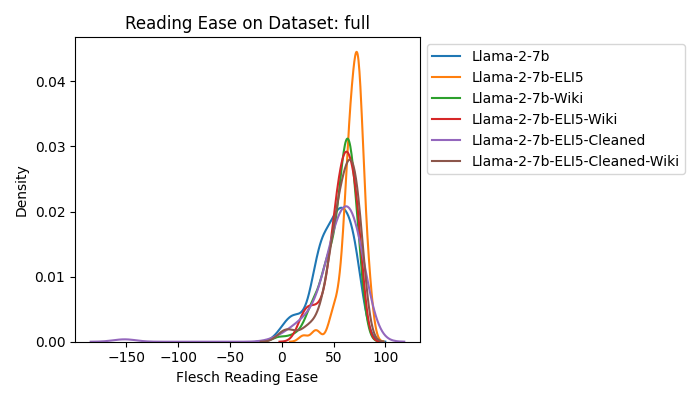
\includegraphics[scale=.5]{./figures/FRE_7B_full.png}
\includegraphics[scale=.5]{./figures/FKG_7B_ELI5.png}
\\
\includegraphics[scale=.5]{./figures/FKG_7B_Wiki.png}
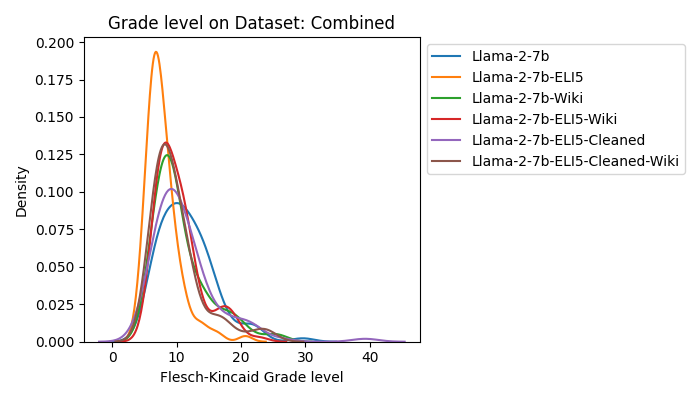
\includegraphics[scale=.5]{./figures/FKG_7B_full.png}
\end{figure}
%\\[10pt]
\noindent\textbf{13B Models}
\\[10pt]
Our analysis of the ROUGE and BERTScores at 13B will closely mirror what we observed at 7B parameters.
In Table \ref{tab:rouge_scores_13B} we see that the base Llama-2 model achieves the highest ROUGE score for all metrics on the ELI5 dataset. In addition, models trained on just the ELI5 dataset appear to achieve the highest ROUGE scores when evaluated on the Simple Wikipedia validation dataset and also perform well when evaluated on the dataset containing questions from both ELI5 and the Simple Wikipedia dataset..
We also again observe that the base Llama-2 model achieves a noticeably higher ROUGELsum score on all three datasets in comparison to our fine-tuned models and that all models perform the best when evaluated on the ELI5 questions.

In Table \ref{tab:bertscores_13B} we also observe that the BERTScores at 13B are similar to those at 7B. 
We see that in many cases the base model achieves the highest BERTScore, but also that the differences between all of the models is relatively small.
Finally, as we before, we observe that all models achieve higher scores on the ELI5 validation set in comparison to the other two sets.
We gain suspect that the models performance, according to these automatic metrics, may be driven more by the pretraining dataset and less by the datasets we fine-tuned on.

\begin{table}[ht]
\centering
\begin{tabular}{lcccccccc}
\toprule
\multicolumn{2}{c}{Dataset} & \multicolumn{1}{c}{rouge1} & \multicolumn{1}{c}{rouge2} & \multicolumn{1}{c}{rougeL} & \multicolumn{1}{c}{rougeLsum} \\
\midrule
\multirow{6}{*}{ELI5} & Llama-2-13b & 0.307 (0.110) & 0.179 (0.119) & 0.232 (0.114) & 0.263 (0.111) \\
& Llama-2-13b-ELI5 & 0.297 (0.100) & 0.152 (0.087) & 0.204 (0.082) & 0.213 (0.085) \\
& Llama-2-13b-Wiki & 0.277 (0.097) & 0.146 (0.090) & 0.193 (0.086) & 0.208 (0.089) \\
& Llama-2-13b-ELI5-Wiki & 0.293 (0.095) & 0.150 (0.085) & 0.203 (0.081) & 0.212 (0.084) \\
& Llama-2-13b-ELI5-Cleaned & 0.296 (0.103) & 0.154 (0.090) & 0.208 (0.086) & 0.217 (0.089) \\
& Llama-2-13b-ELI5-Cleaned-Wiki & 0.293 (0.095) & 0.150 (0.083) & 0.203 (0.079) & 0.213 (0.083) \\
\midrule
\multirow{6}{*}{Wiki} & Llama-2-13b & 0.238 (0.083) & 0.104 (0.067) & 0.166 (0.074) & 0.193 (0.072) \\
& Llama-2-13b-ELI5 & 0.201 (0.057) & 0.069 (0.035) & 0.126 (0.039) & 0.138 (0.043) \\
& Llama-2-13b-Wiki & 0.243 (0.061) & 0.113 (0.043) & 0.166 (0.045) & 0.181 (0.053) \\
& Llama-2-13b-ELI5-Wiki & 0.248 (0.065) & 0.113 (0.045) & 0.170 (0.043) & 0.184 (0.053) \\
& Llama-2-13b-ELI5-Cleaned & 0.210 (0.060) & 0.080 (0.043) & 0.137 (0.050) & 0.150 (0.054) \\
& Llama-2-13b-ELI5-Cleaned-Wiki & 0.246 (0.055) & 0.111 (0.041) & 0.171 (0.039) & 0.184 (0.048) \\
\midrule
\multirow{6}{*}{full} & Llama-2-13b & 0.254 (0.080) & 0.118 (0.081) & 0.177 (0.079) & 0.207 (0.077) \\
& Llama-2-13b-ELI5 & 0.227 (0.077) & 0.091 (0.071) & 0.147 (0.070) & 0.157 (0.072) \\
& Llama-2-13b-Wiki & 0.253 (0.075) & 0.120 (0.069) & 0.173 (0.067) & 0.186 (0.067) \\
& Llama-2-13b-ELI5-Wiki & 0.262 (0.075) & 0.122 (0.068) & 0.179 (0.063) & 0.190 (0.065) \\
& Llama-2-13b-ELI5-Cleaned & 0.227 (0.079) & 0.092 (0.070) & 0.148 (0.068) & 0.159 (0.070) \\
& Llama-2-13b-ELI5-Cleaned-Wiki & 0.262 (0.080) & 0.121 (0.064) & 0.176 (0.062) & 0.188 (0.065) \\
\bottomrule
\end{tabular}
\caption{ROUGE Scores at 13B}
\label{tab:rouge_scores_13B}
\end{table}

\begin{table}[ht]
\centering
\begin{tabular}{lccccccc}
\toprule
Dataset& Model Name  & Precision & Recall & F1 \\
\midrule
\multirow{6}{*}{ELI5} & Llama-2-13b & 0.809 (0.043) & 0.867 (0.036) & 0.837 (0.031) \\
& Llama-2-13b-ELI5 & 0.799 (0.033) & 0.876 (0.034) & 0.835 (0.026) \\
& Llama-2-13b-Wiki & 0.799 (0.032) & 0.873 (0.035) & 0.834 (0.026) \\
& Llama-2-13b-ELI5-Wiki & 0.799 (0.033) & 0.875 (0.034) & 0.834 (0.026) \\
& Llama-2-13b-ELI5-Cleaned & 0.797 (0.034) & 0.875 (0.034) & 0.834 (0.028) \\
& Llama-2-13b-ELI5-Cleaned-Wiki & 0.801 (0.033) & 0.876 (0.034) & 0.836 (0.027) \\
\midrule
\multirow{6}{*}{Wiki} & Llama-2-13b & 0.791 (0.047) & 0.849 (0.033) & 0.818 (0.035) \\
& Llama-2-13b-ELI5 & 0.774 (0.032) & 0.847 (0.025) & 0.808 (0.024) \\
& Llama-2-13b-Wiki & 0.796 (0.026) & 0.886 (0.022) & 0.838 (0.020) \\
& Llama-2-13b-ELI5-Wiki & 0.800 (0.020) & 0.887 (0.022) & 0.841 (0.017) \\
& Llama-2-13b-ELI5-Cleaned & 0.773 (0.041) & 0.848 (0.025) & 0.808 (0.030) \\
& Llama-2-13b-ELI5-Cleaned-Wiki & 0.798 (0.023) & 0.885 (0.024) & 0.839 (0.019) \\
\midrule
\multirow{6}{*}{full} & Llama-2-13b & 0.795 (0.036) & 0.862 (0.029) & 0.827 (0.026) \\
& Llama-2-13b-ELI5 & 0.775 (0.036) & 0.862 (0.029) & 0.816 (0.027) \\
& Llama-2-13b-Wiki & 0.800 (0.028) & 0.889 (0.026) & 0.842 (0.023) \\
& Llama-2-13b-ELI5-Wiki & 0.801 (0.027) & 0.889 (0.026) & 0.842 (0.021) \\
& Llama-2-13b-ELI5-Cleaned & 0.775 (0.041) & 0.863 (0.030) & 0.815 (0.033) \\
& Llama-2-13b-ELI5-Cleaned-Wiki & 0.801 (0.025) & 0.891 (0.024) & 0.843 (0.020) \\
\bottomrule
\end{tabular}
\caption{BERTScores at 13B}
\label{tab:bertscores_13B}
\end{table}




%\end{table}

Next, in Table \ref{tab:FRE_FKG_13B} we look at the Flesch-Kincaid readability metrics for the 13B models. 
We observe again the our fine-tuned models generally have a higher Flesch Readability ease score and a lower Flesch-Kincaid grade level.
However, again there are some exceptions to this rule.
In particular, for all three datasets the model trained on just Simple Wikipedia QA pairs has a lower FRE score and a higher FKG level, so according to both metrics this text is more ``complex".
This may not be entirely surprising, Simple Wikipedia articles are still written in a more dry and more formal style than Reddit posts, and articles may not always be written in a simple way. 
It would be interesting to see if this trend continues to even larger models, i.e. if we trained a 70B model on just the Simple Wikipedia QA pairs would it still be worse than the base 13B models, according to these two metrics, or would the trend reverse?

\begin{figure}
\includegraphics[scale=.5]{./figures/FRE_13B_ELI5.png}
\includegraphics[scale=.5]{./figures/FRE_13B_Wiki.png}
\\
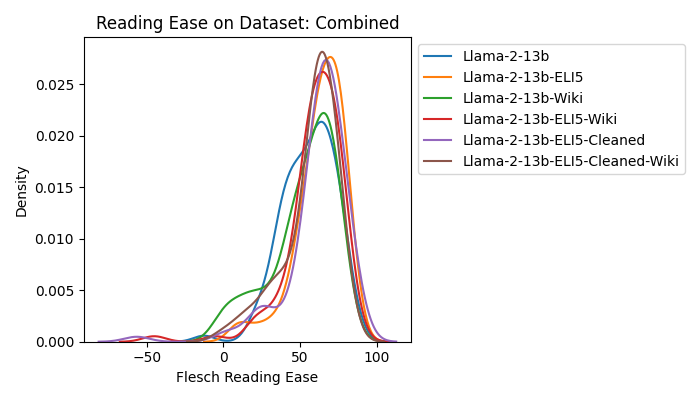
\includegraphics[scale=.5]{./figures/FRE_13B_full.png}
\includegraphics[scale=.5]{./figures/FKG_13B_ELI5.png}
\\
\includegraphics[scale=.5]{./figures/FKG_13B_Wiki.png}
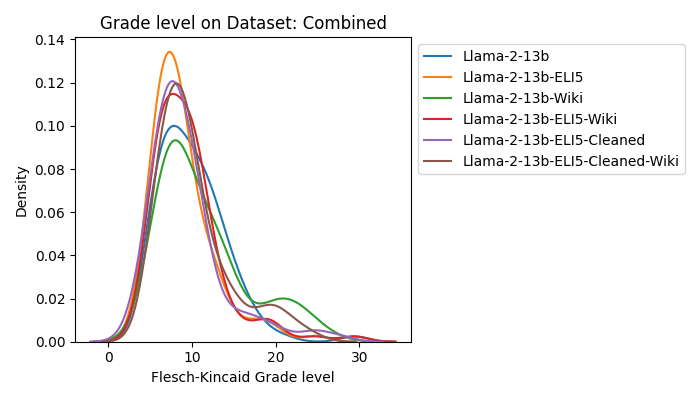
\includegraphics[scale=.5]{./figures/FKG_13B_full.png}
\end{figure}



\begin{table}[h]
\centering
\begin{tabular}{cccc}
\toprule
Dataset & Model Name & FRE & FKG \\
\midrule
ELI5 & Llama-2-13b & 55.9093 & 9.932 \\
 & Llama-2-13b-ELI5 & 55.9616 & 10.142 \\
 & Llama-2-13b-Wiki & 43.5825 & 13.763 \\
  & Llama-2-13b-ELI5-Wiki & 64.5636 & 8.433 \\
 & Llama-2-13b-ELI5-Cleaned & 62.4666 & 8.907 \\
 & Llama-2-13b-ELI5-Cleaned-Wiki & 61.6679 & 9.298 \\
\midrule
Wiki & Llama-2-13b & 55.7939 & 9.999 \\
 & Llama-2-13b-ELI5 & 67.1027 & 7.994 \\
 & Llama-2-13b-Wiki & 51.8992 & 11.595 \\
  & Llama-2-13b-ELI5-Wiki & 60.8368 & 9.324 \\
 & Llama-2-13b-ELI5-Cleaned & 67.8129 & 7.885 \\
 & Llama-2-13b-ELI5-Cleaned-Wiki & 57.7417 & 9.913 \\
 \midrule
Full & Llama-2-13b & 55.5964 & 10.028 \\
 & Llama-2-13b-ELI5 & 63.1428 & 8.895 \\
 & Llama-2-13b-Wiki & 52.3647 & 11.296 \\
  & Llama-2-13b-ELI5-Wiki & 59.5139 & 9.501 \\
 & Llama-2-13b-ELI5-Cleaned & 61.2361 & 9.339 \\
 & Llama-2-13b-ELI5-Cleaned-Wiki & 56.9492 & 10.218 \\
\bottomrule
\end{tabular}
\caption{FRE and FKG Scores at 13B}
\label{tab:FRE_FKG_13B}
\end{table}



\subsubsection{Judging the Validation Set with GPT-4}
Finally, its time to move away from the world of automatic metrics and start to consider more fine-grained and intelligent ways to evaluate the output of generative models.
One option is to crowdsource this problem to human volunteers and ask them to rank or score various model's responses.
An alternative, and faster option, is to ask an intelligent AI, such as GPT-4, to score the model responses. 
This is the approach we will take in this section, namely we will simply ask GPT-4 to assign a score to each answer according to a custom prompt.
Inspired by the prompt used in MT-bench \cite{zheng2023judging}, we decided to prompt GPT-4 as follows:
\\
\begin{displayquote}
$[$Instruction$]$\newline Please act as an impartial judge and
    evaluate the quality of the response provided by an AI assistant
    to the user question displayed below. Your evaluation should consider
    factors such as the following:\newline\newline- **Simplicity**: Is the response
    clear and straightforward enough for middle or high school students to
    understand?\newline- **Helpfulness**: Does the response effectively address
    the query?\newline- **Relevance**: Does the response directly pertain to the
    question?\newline- **Accuracy**: Is the response factually correct?\newline-
    **Depth \& Creativity**: Assess richness without favoring excessive
    detail.\newline\newline Aim for a holistic assessment. Begin your evaluation by
    providing a short explanation. Be as objective as possible. After
    providing your explanation, you must rate the response on a scale
    of 1 to 10 by strictly following this format: `[[rating]]',
    for example: `Rating: [[5]]'.\newline\newline[Question]\newline{\{question\}}\newline\newline
    [The Start of Assistant's Answer]\newline{\{answer\}}\newline[The End of Assistant's
    Answer]
\end{displayquote}

Here the text in \{question\} and \{answer\} correspond to the question in one of our datasets and the model generated answer, respectively.
Given that GPT-4 is not cheap, we decided to only evaluate our models on the small validation set containing 100 questions from both ELI5 and Simple Wikipedia.

\begin{table}[h]
\centering
\begin{tabular}{|l|c|}
\hline
Model Name & Score \\
\hline
Llama-2-7b-ELI5-Cleaned-Wiki & 3.89 \\
Llama-2-7b-Wiki & 3.58 \\
Llama-2-7b-ELI5-Wiki & 3.45 \\
Llama-2-7b & 2.92 \\
Llama-2-7b-ELI5-Cleaned & 2.58 \\
Llama-2-7b-ELI5 & 2.43 \\
\hline\hline 
Llama-2-13b-ELI5-Wiki & 4.91 \\
Llama-2-13b-ELI5-Cleaned-Wiki & 4.77 \\
Llama-2-13b-Wiki & 4.53 \\
Llama-2-13b & 3.43 \\
Llama-2-13b-ELI5-Cleaned & 3.27 \\
Llama-2-13b-ELI5 & 3.17 \\
\hline
\end{tabular}
\caption{GPT-4 judgements at 7B and 13B}
\label{tab:GPT4-judgements}
\end{table}
  
In Table \ref{tab:GPT4-judgements} we present the average scores assigned by GPT-4 to each model, ranked for highest to lowest.
We also separated the results by the size of the model.
At both 7B and 13B, the three best performing models are the ones trained on ELI5 + Simple Wikipedia (using our original ELI5 SFT dataset or the cleaned one) and the one trained on just Simple Wikipedia.
By contrast, the model trained on just ELI5 performs worse than the base model at both 7B and 13B.
We think these results indicate that training on the more encyclopedic text of Simple Wikipedia helps the model generate more cogent answers.







%\subsubsection{MT(S)-Bench}
%
%In this section we will investigate how well our models perform on a new MT-bench like dataset.
%The idea of MT-bench is to use a LLM, like GPT-4, to judge the output of other, smaller LLMs. 
%There are two types of completion tasks, single-turn and multi-turn.
%For a single-turn problem, the model is given a prompt and asked to complete it.
%For a multi-turn problem, the model is prompted with one complete turn of a conversation (i.e. question and answer) and then asked to reply to a new, follow-up question. 
%Given that our models are only trained for single-turn problems, we will see that they do not perform well on multi-turn problems.
%
%\begin{center}
%\begin{tabular}{c|c|c}
%    \hline
%    \textbf{Model} & \textbf{Single-Turn score}& \textbf{Multi-Turn score} \\
%    \hline
%    Llama-2-7b-chat &  9.40 & 8.80\\ 
%    Llama-2-7b-ELI5-Wiki-simple-merge & 6.683333 & 3.533333  \\
%    Llama-2-7b-ELI5-Wiki &  5.975000 &  2.966667 \\
%    Llama-2-7b-Wiki &  5.108333 & 1.616667  \\
%    Llama-2-7b-ELI5 &  4.116667 & 1.733333  \\
%    Llama-2-7b-Wiki-simple-merge &  2.300000& 1.033333  \\
%    Llama-2-7b-ELI5-simple-merge & 2.000000 & 1.200000  \\
%    Llama-2-7b & 1.066667 &1.000000 \\
%    \hline
%\end{tabular}
%\end{center}
%
%Next let's look at the readability scores of each model on the single prompt:
%
%\begin{center}
%\begin{tabular}{c|c|c}
%    \hline
%    \textbf{Model} & \textbf{FRE}& \textbf{FKG} \\
%    \hline
%    Llama-2-7b-chat &  42.21 & 12.50 \\ 
%    Llama-2-7b-ELI5-Wiki-simple-merge & 60.55 & 9.60  \\
%    Llama-2-7b-ELI5-Wiki &  53.41 &  10.20 \\
%    Llama-2-7b-Wiki &  91.41 & 3.90 \\
%    Llama-2-7b-ELI5 &  63.19 & 8.50 \\
%    Llama-2-7b-Wiki-simple-merge &  96.48& 2.00  \\
%    Llama-2-7b-ELI5-simple-merge & 78.65 & 4.70  \\
%    Llama-2-7b & 29.86 &13.10 \\
%    \hline
%\end{tabular}
%\end{center}
%
%



\newpage
\bibliographystyle{utphys}
\bibliography{refs}


\end{document}  